\documentclass[a4paper, 12pt]{scrreprt}
\usepackage[left = 2.5cm,right = 2cm,bottom = 4cm]{geometry}
\usepackage[onehalfspacing]{setspace}
\usepackage[
	pdftitle={Dokumentation kürzeste Pfade},
	pdfsubject={},
	pdfauthor={Robin Meier, Stefan Manthey},
	pdfkeywords={},
	hidelinks
]{hyperref}

\usepackage[utf8]{inputenc}
\usepackage[ngerman]{babel}
\usepackage[T1]{fontenc}
\usepackage{graphicx,subfig}
\graphicspath{{img/}}
\usepackage{fancyhdr}
\usepackage{lmodern}
\usepackage{color}
\usepackage{amsfonts}
\usepackage{amsmath}
\usepackage{listings}
\usepackage{xcolor}
\usepackage[subfigure]{tocloft}
\usepackage{hyperref}
\fontfamily{vna}\selectfont

\definecolor{dkgreen}{rgb}{0,0.6,0}
\definecolor{gray}{rgb}{0.5,0.5,0.5}
\definecolor{mauve}{rgb}{0.58,0,0.82}

\lstdefinestyle{mystyle}{
	numbers=left,
	frame=single,
	basicstyle=\small,
	numbers=left,
	numberstyle=\tiny,
	numbersep=15pt,tabsize=4,
	flexiblecolumns=true,
	keywordstyle=\color{blue},
	commentstyle=\color{dkgreen}, 
	stringstyle=\color{mauve},
	numberstyle=\tiny\color{gray},
	language=Java,
	breaklines=true,
	breakatwhitespace=true,
	morekeywords={*,num,String,var,library,get,set}
}

\lstset{style=mystyle}

\usepackage[backend=bibtex, style=numeric]{biblatex}
%\addbibresource{Literatur.bib}

\pagestyle{fancy}
\lhead{}
\chead{}
\rhead{\slshape \leftmark}

\lfoot{}
\cfoot{\thepage}
\rfoot{}

\renewcommand{\headrulewidth}{0.4pt}
\renewcommand{\footrulewidth}{0pt}

\begin{document}

\pagestyle{empty}
\pagenumbering{Roman}

\begin{center}
\begin{tabular}{p{\textwidth}}

\begin{center}

\includegraphics[scale=1.5]{img/HTW_Berlin_Logo_farbig.jpg}
\end{center}

\\

\begin{center}
\LARGE{\textsc{
CIRS APP
}}
\end{center}

\\

\begin{center}
\large{
Dokumentation der mobilen Critical Incedent Reporting System App
}
\end{center}

\\

\begin{center}
\textbf{\large{Dokumentation}}
\end{center}

\begin{center}
vorgelegt von
\end{center}

\begin{center}
\large{\textbf{Amanda Joelle Dzukou Kom}} \\
\large{\textbf{Stefan Manthey}} \\
\large{\textbf{Michael Pientka}}
\end{center}

\begin{center}
geschrieben von
\end{center}

\begin{center}
Stefan Manthey
\end{center}

\begin{center}
\large{27.01.2021}
\end{center}

\\

\\

\end{tabular}
\end{center}

\cleardoubleoddpage
\pagestyle{fancy}

\renewcommand{\cftpartleader}{\cftdotfill{\cftdotsep}} % for parts
\renewcommand{\cftchapleader}{\cftdotfill{\cftdotsep}} % for chapters
\renewcommand{\cftsecleader}{\cftdotfill{\cftdotsep}} % for sections
\tableofcontents
\newpage
\listoffigures
\newpage
%\listoftables
%\newpage
\lstlistoflistings
\newpage

%Hier die Inhalte inkludieren
\pagenumbering{arabic}
\chapter{Entwickler Dokumentation}
\label{entw_docu}
In dem folgenden Kapitel wird die Einrichtung, zur Benutzung der CIRS-APP, beschrieben. Dabei werden sowohl die notwendigen Software Tools genannt, als auch die Nutzung zum starten der APP auf einem Android Emulator und einem Android Smartphone.

\section{Voraussetzungen}
\label{voraussertungen}
Für die Nutzung der App wird ein Backend Server benötigt. Um die Server Software auszuführen benötigen Sie:
\begin{itemize}
\item Node.js, hier zu finden \url{https://nodejs.org/en/} (die LTS Version ist zu bevorzugen)
\item Git
\end{itemize}
Für die Kompelierung der App benötigen Sie die folgenden Software-Tools:
\begin{itemize}
\item Flutter SDK, hier zu finden \url{https://flutter.dev/docs/get-started/install}
\item Git
\item JDK 8, hier zu finden \url{https://www.oracle.com/de/java/technologies/javase/javase-jdk8-downloads.html}
\item Android Studio, dies kann zusammen mit dem Android Studio heruntergeladen werden \url{https://developer.android.com/studio}
\item 
\end{itemize}
Laden Sie die Backend Server Software vom Github-Repository \url{https://github.com/amandajoelle/Backend} herunter. Sie können diese als Zip-Datei herunterladen oder mit dem Befehl \textit{git clone https://github.com/amandajoelle/Backend.git}.\\
Laden Sie sich anschließend die CIRS-APP herunter, vom Github-Repository \url{https://github.com/amandajoelle/Frontend}.

\section{Benutzung}
\label{benutzung}
Zuerst müssen die benötigten Abhängigkeiten heruntergeladen werden, hierfür muss der Befehl \textit{npm install} im Ordner Backend ausgeführt werden. Erstellen Sie im Backend-Ordner eine \textit{.env} Datei. Diese sollte mit Umgebungsvariablen initialisiert werden. Dies können Sie der README.md entnehmen.\\
Anschließend muss die Datenbank erstellt werden. Mithilfe des Befehles \textit{npm run database} wird eine Datenbank im Unterordner \textit{database} erstellt. Hier befindet sich nun die Datei \textit{cirs.db}, welche alle Datenbankeinträge beinhaltet. Abschließend muss die Backend Server Software nur noch mit dem Kommando \textit{npm run dev} gestartet werden.
\\[0.5cm]
Für die Kompilierung und Nutzung der CIRS-APP in einem Android Emulator, installieren Sie Android Studio und fügen Sie dem AVD einen Emulator hinzu.
\begin{figure}[hbt!]
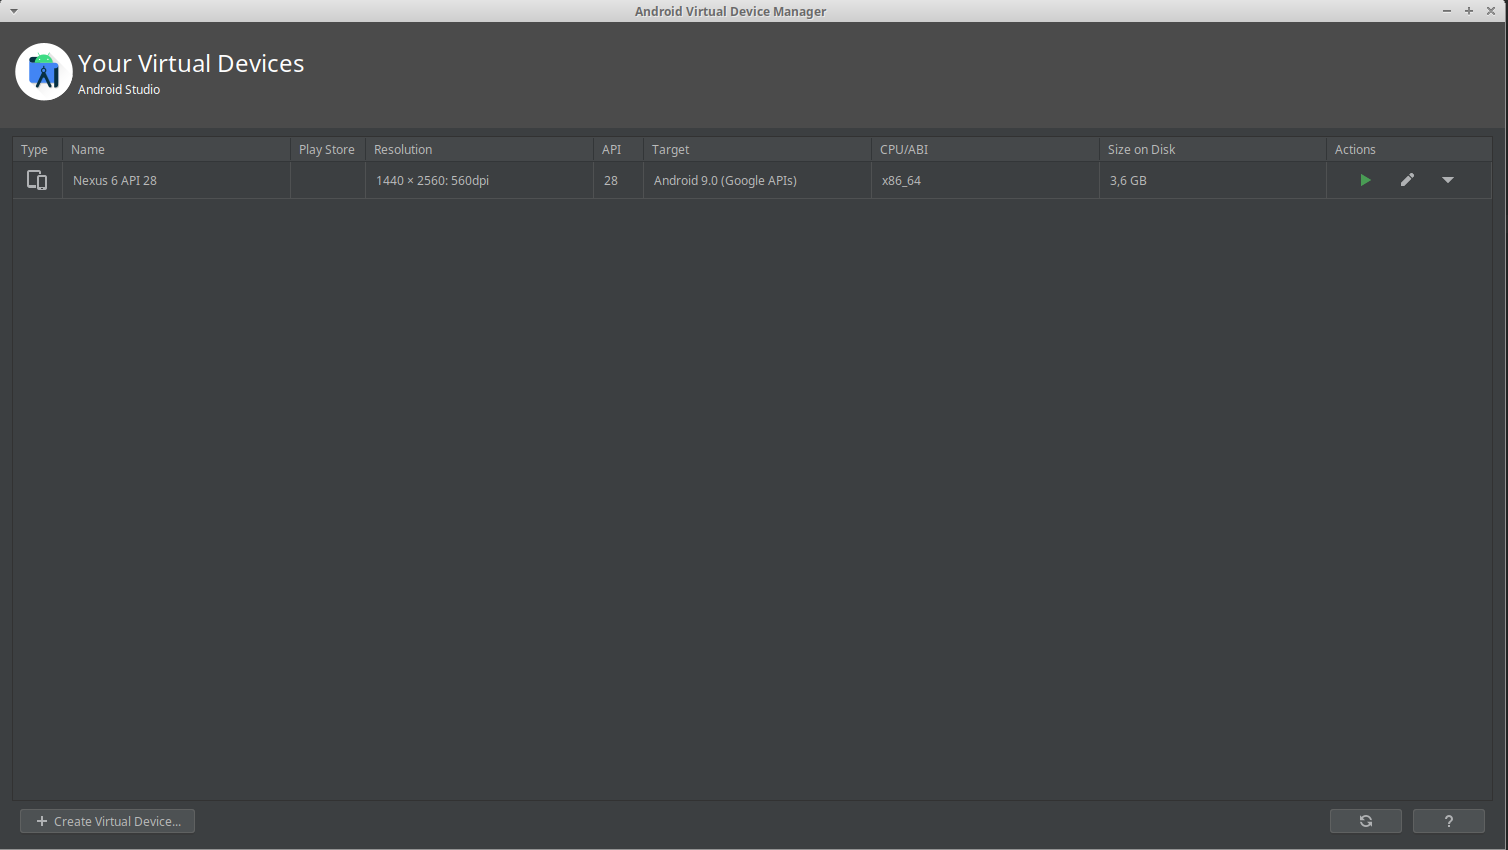
\includegraphics[width=16cm]{AVD.png}
\caption{AVD Menü zum erstellen und starten von Android Emulatoren}
\label{fig:avd}
\end{figure}
Starten Sie den Android Emulator und für Sie in einem Terminal, im Frontend Ordner, den Befehl \textit{flutter run --release} aus.
\\[0.5cm]
Im Login Bildschirm der App, können Sie ich mit einem Beispiel Nutzer anmelden, um Fälle zu bearbeiten. Die Zugangsdaten sind:
\begin{itemize}
\item E-Mail: Mueller@cirs.de
\item Passwort: 123456789
\end{itemize}
Die App kann ebenfalls auf einem Android Smartphone ausgeführt werden. Hierfür muss in der Datei \textit{main.dart}, im Verzeichnis \textit{frontend/lib} die ServerUrl geändert werden.
\begin{lstlisting}[language=Java, caption=ServerUrl ersetzen, label=lst:url_ersetzen]
...
final String serverUrl = 'http://10.0.2.2:8080';

void main() {
  runApp(MaterialApp(home: MyApp()));
}
...
\end{lstlisting}
Ersetzen Sie die IP Adresse in der Konstanten \textit{serverUrl}, aus dem Listing \ref{lst:url_ersetzen}, für die Ihres Computers auf dem die Backend Server Software ausgeführt wird. Sowohl \textit{http://} als auch \textit{:8080} müssen Bestandteil der URL bleiben.



%Literaturverzeichnis
%\printbibliography[
%heading=bibintoc,
%title={Quellenverzeichnis}
%]

\end{document}
